\fancyhead[LE]{\fontsize{8.5pt}{10pt}\selectfont\textbf{\textsf{\thepage}}\quad \textbf{\textsf{CHƯƠNG 1}}\quad \textsf{Các hàm số và Mô hình}}
\fancyhead[RO]{\fontsize{8.5pt}{10pt}\selectfont\textsf{MỤC 1.5}\quad \textbf{\textsf{\thepage}}}

\noindent
\begin{minipage}[t]{0.265\textwidth}
    \fontsize{8pt}{10.5pt}\selectfont
    \vspace*{4.8cm}
    
    Trong Ví dụ 4, hãy chú ý cách $f^{-1}$ đảo ngược tác động của $f$. Hàm số $f$ là quy tắc “Lập phương, sau đó cộng 2”; còn $f^{-1}$ là quy tắc “Trừ đi 2, sau đó lấy căn bậc ba”.

    \vspace{6.2cm}
    \centering
    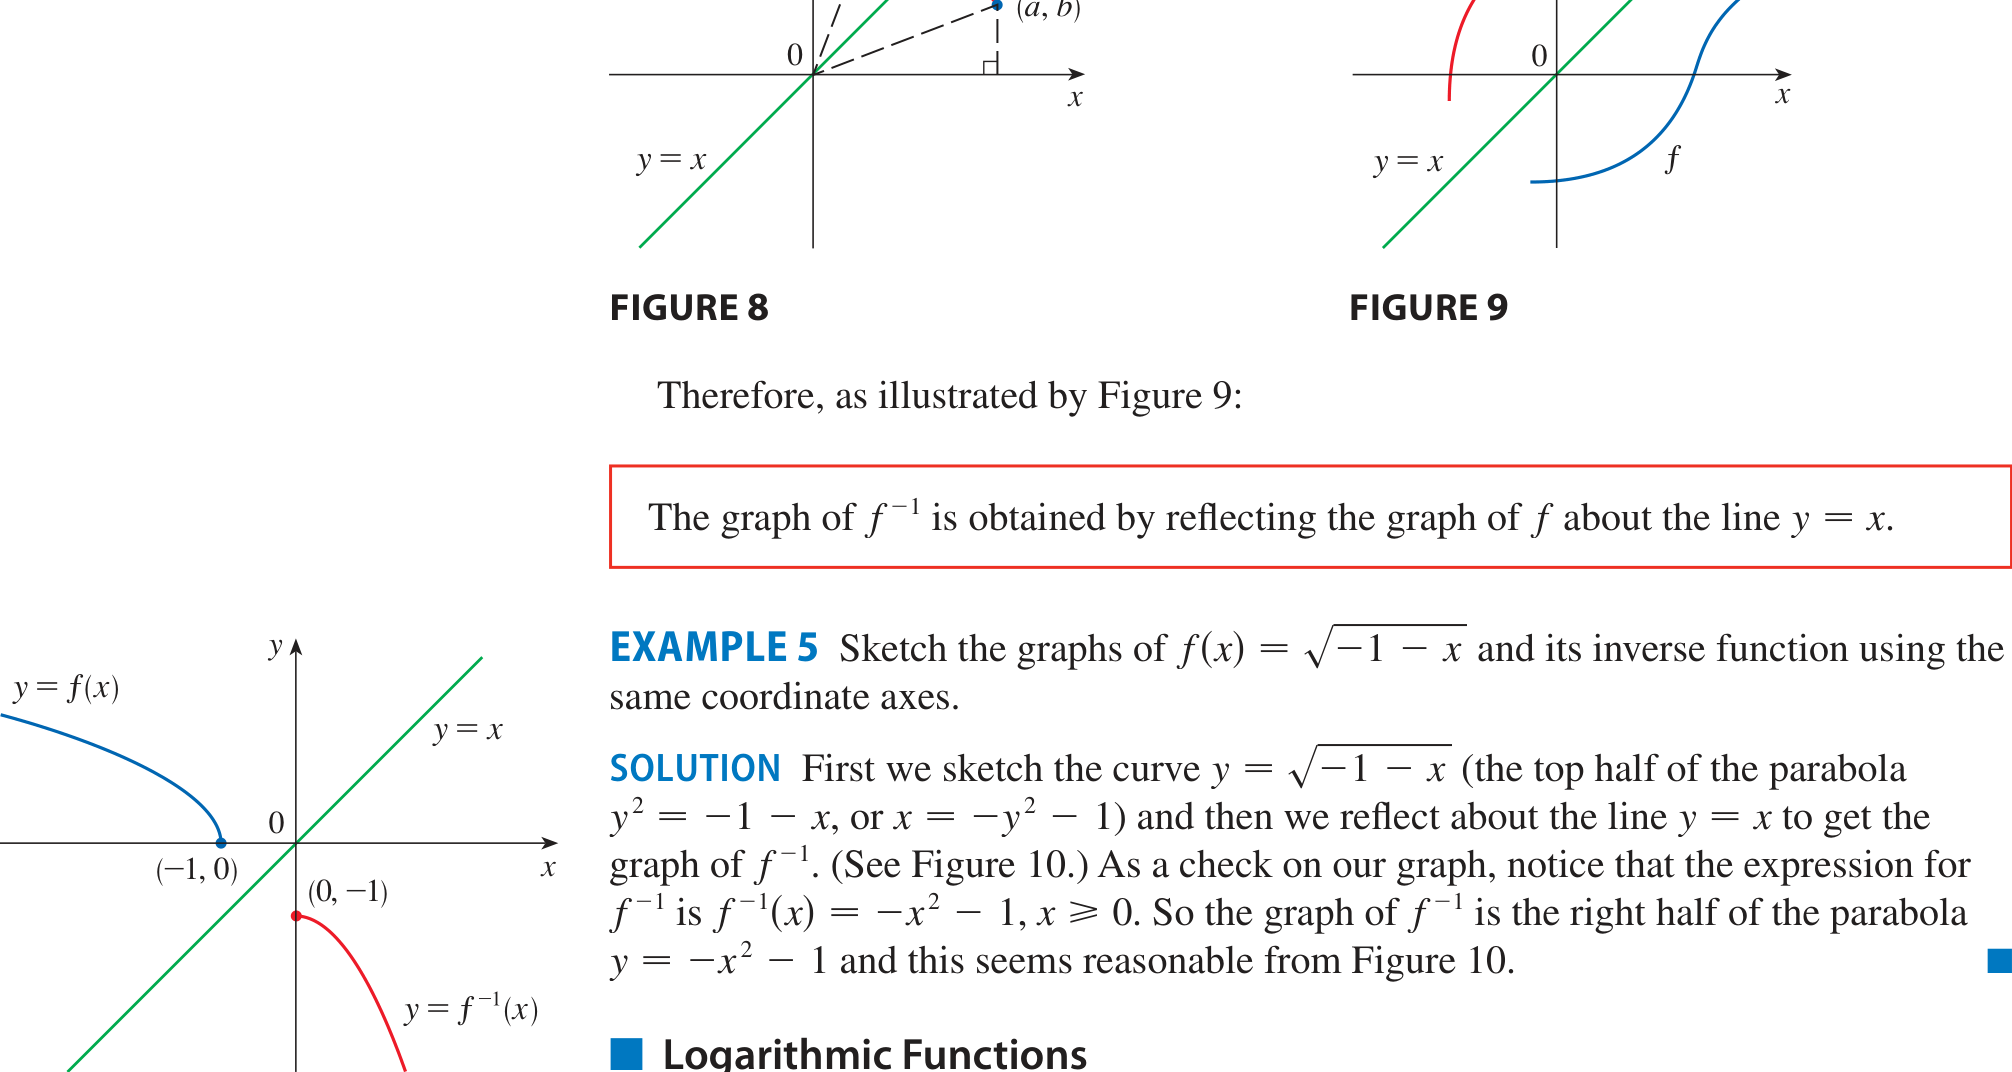
\includegraphics[width=0.92\linewidth]{images/p0092_fig10.png}
    \vspace{0.3em}

    \textbf{\textsf{HÌNH 10}}
\end{minipage}%
\hfill
\begin{minipage}[t]{0.708\textwidth}
    \fontsize{9.3pt}{13.2pt}\selectfont
    \noindent\textbf{\textsf{\color{stewartcyan}VÍ DỤ 4}}\quad Tìm hàm số ngược của $f(x) = x^3 + 2$.

    \vspace{0.2em}
    \noindent\textbf{\textsf{\color{stewartcyan}LỜI GIẢI}}\quad Theo (5), trước tiên ta viết
    \[
    y = x^3 + 2
    \]
    Sau đó ta giải phương trình này theo $x$:
    \begin{align*}
    x^3 &= y - 2\\[3pt]
    x &= \sqrt[3]{y - 2}
    \end{align*}
    Cuối cùng, ta hoán đổi $x$ và $y$:
    \[
    y = \sqrt[3]{x - 2}
    \]
    Do đó, hàm số ngược là $f^{-1}(x) = \sqrt[3]{x - 2}$.\hfill{\color{stewartcyan}$\blacksquare$}

    \vspace{0.8em}
    Nguyên tắc hoán đổi $x$ và $y$ để tìm hàm số ngược cũng cung cấp cho chúng ta phương pháp xác định đồ thị của $f^{-1}$ từ đồ thị của $f$. Vì $f(a) = b$ khi và chỉ khi $f^{-1}(b) = a$, nên điểm $(a, b)$ nằm trên đồ thị của $f$ khi và chỉ khi điểm $(b, a)$ nằm trên đồ thị của $f^{-1}$. Nhưng ta thu được điểm $(b, a)$ từ $(a, b)$ bằng cách lấy đối xứng qua đường thẳng $y = x$. (Xem Hình 8.)

    \begin{center}
    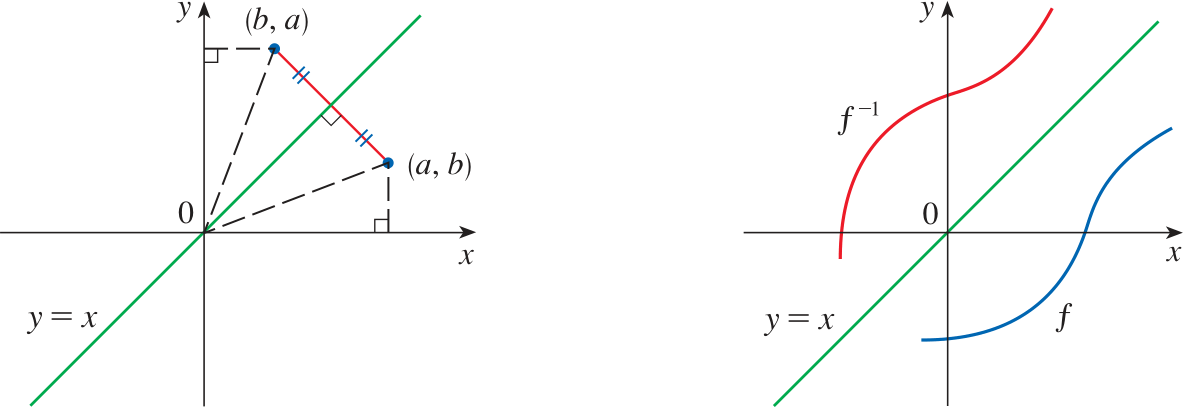
\includegraphics[width=0.85\linewidth]{images/p0092_fig8.png}
    \end{center}

    Do đó, như được minh họa ở Hình 9:

    \begin{definitionbox}
    Đồ thị của $f^{-1}$ nhận được bằng cách lấy đối xứng đồ thị của $f$ qua đường thẳng $y = x$.
    \end{definitionbox}

    \vspace{0.8em}
    \noindent\textbf{\textsf{\color{stewartcyan}VÍ DỤ 5}}\quad Vẽ đồ thị của hàm số $f(x) = \sqrt{-1 - x}$ và hàm số ngược của nó trên cùng một hệ trục tọa độ.

    \vspace{0.2em}
    \noindent\textbf{\textsf{\color{stewartcyan}LỜI GIẢI}}\quad Trước tiên, ta vẽ đường cong $y = \sqrt{-1 - x}$ (nửa trên của parabol $y^2 = -1 - x$, hay $x = -y^2 - 1$), sau đó ta lấy đối xứng qua đường thẳng $y = x$ để nhận được đồ thị của $f^{-1}$. (Xem Hình 10.) Để kiểm tra lại đồ thị, hãy lưu ý rằng biểu thức của $f^{-1}$ là $f^{-1}(x) = -x^2 - 1$, $x \ge 0$. Do đó, đồ thị của $f^{-1}$ là nửa bên phải của parabol $y = -x^2 - 1$, và điều này hoàn toàn hợp lý khi quan sát Hình 10.\hfill{\color{stewartcyan}$\blacksquare$}

    \vspace{1.2em}
    \noindent{\color{stewartcyan}\rule{1.1ex}{1.1ex}}\hspace{0.5em}\textbf{\textsf{\large Các hàm số Lôgarit}}

    \vspace{0.4em}
    Nếu $b > 0$ và $b \ne 1$, hàm số mũ $f(x) = b^x$ luôn đồng biến hoặc luôn nghịch biến, và do đó nó là đơn ánh theo Kiểm tra đường thẳng nằm ngang. Vì thế nó có hàm số ngược $f^{-1}$, được gọi là \textbf{hàm số lôgarit cơ số $b$} và được ký hiệu là $\log_b$. Nếu ta dùng định nghĩa hàm số ngược được cho bởi (3), thì
    \[
    f^{-1}(x) = y \iff f(y) = x
    \]
\end{minipage}